\documentclass[student,noshadow]{ITRslides}
\usepackage{multimedia}

\usepackage[absolute,overlay]{textpos}
\renewcommand{\vec}[1]{\boldsymbol{#1}}
\addbibresource{ref.bib}
\graphicspath{{pics/}{logos/}}
\usepackage{psfrag}
\usepackage[percent]{overpic}
\usepackage{subcaption}
\usepackage{units}
\usepackage{tikz}
\usetikzlibrary{positioning,shapes,fadings,decorations.pathmorphing,arrows}
\title{Object exploration using visual/haptic information by a human-robot team}
\presenter{Florian Wirnshofer, Benedikt Schmidt}

\supervisor{Denis Cehajic}
\typeofpres{Project Laboratory Cognitive Robotics and Control}

\definecolor{light-gray}{gray}{0.95}

\newcommand*\MyBlue{%
  \item[\color{blue}\scalebox{0.9}{\textbullet}]}
\newcommand*\MyRed{%
  \item[\color{red}\scalebox{0.9}{\textbullet}]}
%\nocite{*}

\renewcommand{\vec}[1]{\boldsymbol{#1}} 
% Alle indizes in Normalschrift ausser Läuferindizes
\newcommand{\scr}[1]{\mathrm{#1}} 

\makeatletter
\newif\iftikz@shading@path

\tikzset{
    % There are three circumstances in which the fading sep is needed:
    % 1. Arrows which do not update the bounding box (which is most of them).
    % 2. Line caps/joins and mitres that extend outside the natural bounding 
    %    box of the path (these are not calculated by PGF).
    % 3. Other reasons that haven't been anticipated.
    fading xsep/.store in=\pgfpathfadingxsep,
    fading ysep/.store in=\pgfpathfadingysep,
    fading sep/.style={fading xsep=#1, fading ysep=#1},
    fading sep=0.0cm,
    shading path/.code={%
        % Prevent this stuff happning recursively.
        \iftikz@shading@path%
        \else%
            \tikz@shading@pathtrue%
            % \tikz@addmode installs the `modes' (e.g., fill, draw, shade) 
            % to be applied to the path. It isn't usualy for doing more
            % changes to the path's construction.
            \tikz@addmode{%
                \pgfgetpath\pgf@currentfadingpath%
                % Get the boudning box of the current path size including the fading sep
                \pgfextract@process\pgf@fadingpath@southwest{\pgfpointadd{\pgfqpoint{\pgf@pathminx}{\pgf@pathminy}}%
                    {\pgfpoint{-\pgfpathfadingxsep}{-\pgfpathfadingysep}}}%%
                \pgfextract@process\pgf@fadingpath@northeast{\pgfpointadd{\pgfqpoint{\pgf@pathmaxx}{\pgf@pathmaxy}}%
                    {\pgfpoint{\pgfpathfadingxsep}{\pgfpathfadingysep}}}%
                % Clear the path
                \pgfsetpath\pgfutil@empty%                          
                % Interrupt the path and picture to create a fading.
                \pgfinterruptpath%
                \pgfinterruptpicture%
                    \begin{tikzfadingfrompicture}[name=.]
                        \path [shade=none,fill=none, #1] \pgfextra{%
                            % Set the softpath. Any transformations in #1 will have no effect.
                            % This will *not* update the bounding box...
                            \pgfsetpath\pgf@currentfadingpath%
                            % ...so it is done manually.
                            \pgf@fadingpath@southwest
                            \expandafter\pgf@protocolsizes{\the\pgf@x}{\the\pgf@y}%
                            \pgf@fadingpath@northeast%
                            \expandafter\pgf@protocolsizes{\the\pgf@x}{\the\pgf@y}%
                        };
                        % Now get the bounding of the picture.
                        \xdef\pgf@fadingboundingbox@southwest{\noexpand\pgfqpoint{\the\pgf@picminx}{\the\pgf@picminy}}%
                        \xdef\pgf@fadingboundingbox@northeast{\noexpand\pgfqpoint{\the\pgf@picmaxx}{\the\pgf@picmaxy}}%
                        %
                    \end{tikzfadingfrompicture}%
                \endpgfinterruptpicture%
                \endpgfinterruptpath%
                % Install a rectangle that covers the shaded/faded path picture.                                
                \pgfpathrectanglecorners{\pgf@fadingboundingbox@southwest}{\pgf@fadingboundingbox@northeast}%
                % Make the fading happen.
                \def\tikz@path@fading{.}%
                \tikz@mode@fade@pathtrue%
                \tikz@fade@adjustfalse%10pt
                % Shift the fading to the mid point of the rectangle
                \pgfpointscale{0.5}{\pgfpointadd{\pgf@fadingboundingbox@southwest}{\pgf@fadingboundingbox@northeast}}%
                \edef\tikz@fade@transform{shift={(\the\pgf@x,\the\pgf@y)}}%
            }%
        \fi%
    }
}

%%%%%%%%%%%%%%%%%%%%%%%%%%%%%%%%%%%%%%%%%%%%%%%%%%%%%%%%%%%%%%%%%%%%%%%%%%%%%%%%

\begin{document}


\begin{frame}
    \titlepage
\end{frame}

%%%%%%%%%%%%%%%%%%%%%%%%%%%%%%%%%%%%%%%%%%%%%%%%%%%%%%%%%%%%%%%%%%%%%%%%%%%%%%%%
%INTRODUCTION , MOTIVATION
%%%%%%%%%%%%%%%%%%%%%%%%%%%%%%%%%%%%%%%%%%%%%%%%%%%%%%%%%%%%%%%%%%%%%%%%%%%%%%%%
\begin{frame}
	\frametitle{Content}
	\tableofcontents
\end{frame}

\section{Online Load Estimation}
\begin{frame}
	%Benedikt
	\frametitle{Task}
	\begin{block}{Goal}
			Human-Robot cooperative estimation of load uncertainties.
	\end{block}
	\vspace{2mm}
	\begin{block}{Key-Questions}
			\begin{itemize}
				\item How to fuse and process sensor feedback, resulting in a reliable load-identification?
				\item How should the agents excite the load?
				\item How to exchange information between agents?
			\end{itemize}	   
	\end{block}	
\end{frame}

\begin{frame}
	%Florian
	\frametitle{Online Load Estimation}

	\begin{columns}
		\centering
		 	\begin{column}{0.25\textwidth}
			\begin{figure}
			\centering
				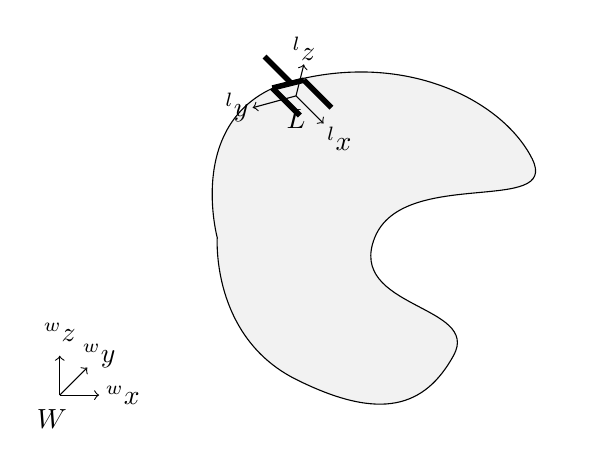
\begin{tikzpicture}
	% world frame
	\draw[arrows=->,line width=0.4pt] (0, 0) -- (0.5, 0);
	\draw[arrows=->,line width=0.4pt] (0, 0) -- (0.35, 0.35);
	\draw[arrows=->,line width=0.4pt] (0, 0) -- (0, 0.5);
	\node at (0.8, 0) {$^wx$};
	\node at (0.5, 0.5) {$^wy$};
	\node at (0, 0.8) {$^wz$};
	\node at (-0.1, -0.3) {$W$};
	
	% load
	\draw[fill,light-gray,draw=black] plot[smooth, tension=1.3] coordinates {(2, 2) (3, 4) (6, 3) (4, 2) (5, 0.5) (3, 0.2) (2, 2)};
	
	% load frame
	\draw[arrows=->,line width=0.4pt] (3, 3.8) -- (3.35, 3.45);
	\draw[arrows=->,line width=0.4pt] (3, 3.8) -- (2.45, 3.65);
	\draw[arrows=->,line width=0.4pt] (3, 3.8) -- (3.1, 4.2);
	\node at (3.55, 3.25) {$^lx$};
	\node at (2.25, 3.65) {$^ly$};
	\node at (3.1, 4.4) {$^lz$};
	\node at (3, 3.5) {$L$};
	
	% gripper
	\draw[draw=black,line width=2pt] (3.1, 4) -- (3.45, 3.65);
	\draw[draw=black,line width=2pt] (2.7, 3.9) -- (3.05, 3.55);
	\draw[draw=black,line width=2pt] (3.1, 4) -- (2.7, 3.9);
	\draw[draw=black,line width=2pt] (2.6, 4.3) -- (2.95, 3.95);
\end{tikzpicture} 
			\end{figure}
		 	\end{column}
		 		
		 	\begin{column}{0.75\textwidth}
			Model:\\ \cite{literaturstelle2}\\
			%\vspace{0.1cm}
			\[^\scr{L}\vec{F} = m {^\scr{W}}\vec{\ddot{p}} + m ^\scr{L}\vec{g} + ^\scr{L}\vec{\dot{\omega}} \times m ^\scr{L}\vec{c} + ^\scr{L}\vec{\omega} \times (^\scr{L}\vec{\omega} \times m ^\scr{L}\vec{c})\]
			\[^\scr{L}\vec{N} = ^\scr{L}\vec{I} ^\scr{L}\vec{\dot{\omega}} + ^\scr{L}\vec{\omega} \times (^\scr{L}\vec{I} ^\scr{L}\vec{\omega}) + m ^\scr{L}\vec{c} \times {^\scr{W}}\vec{\ddot{p}} + m ^\scr{L}\vec{c} \times ^\scr{L}\vec{g}\]
			
			\vspace{0.1cm}
			$\vec{\ddot{p}}$ EEF acceleration\\
			$m$ Object mass\\
			$\vec{I}$  Object inertia tensor
		 	\end{column}
	\end{columns}
	 		\vspace{0.2cm}
			RLS Estimation-Parameters: \\
			$\vec{\Theta} = [m, m c_\scr{x}, m c_\scr{y}, m c_\scr{z}, I_\scr{xx}, I_\scr{xy}, I_\scr{xz}, I_\scr{yy},I_\scr{yz}, I_\scr{zz}]^\scr{T}$ \\
\end{frame}

\begin{frame}
	%Florian
	\frametitle{Cooperative Online Load Estimation}
	\begin{columns}
			\begin{column}{0.5\textwidth}
				\begin{figure}
					\centering
					\resizebox{4cm}{!}{
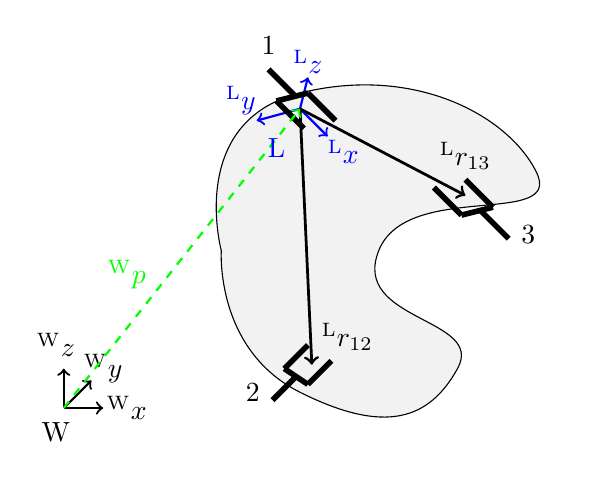
\begin{tikzpicture}
	% world frame
	\draw[arrows=->,line width=0.8pt] (0, 0) -- (0.5, 0);
	\draw[arrows=->,line width=0.8pt] (0, 0) -- (0.35, 0.35);
	\draw[arrows=->,line width=0.8pt] (0, 0) -- (0, 0.5);
	\node at (0.8, 0) {{$^\mathrm{W}x$}};
	\node at (0.5, 0.5) {{$^\mathrm{W}y$}};
	\node at (-0.1, 0.8) {{$^\mathrm{W}z$}};
	\node at (-0.1, -0.3) {W};	
	% load
	\draw[fill,light-gray,draw=black] plot[smooth, tension=1.3] coordinates {(2, 2) (3, 4) (6, 3) (4, 2) (5, 0.5) (3, 0.2) (2, 2)};
	
	% load frame
	\draw[draw=blue,arrows=->,line width=0.8pt] (3, 3.8) -- (3.35, 3.45);
	\draw[draw=blue,arrows=->,line width=0.8pt] (3, 3.8) -- (2.45, 3.65);
	\draw[draw=blue,arrows=->,line width=0.8pt] (3, 3.8) -- (3.1, 4.2);
	\node[text=blue] at (3.55, 3.25) {{$^\mathrm{L}x$}};
	\node[text=blue] at (2.25, 3.9) {{$^\mathrm{L}y$}};
	\node[text=blue] at (3.1, 4.4) {{$^\mathrm{L}z$}};
	
		
	
	
	% gripper one
	\draw[draw=black,line width=2pt] (3.1, 4) -- (3.45, 3.65);
	\draw[draw=black,line width=2pt] (2.7, 3.9) -- (3.05, 3.55);
	\draw[draw=black,line width=2pt] (3.1, 4) -- (2.7, 3.9);
	\draw[draw=black,line width=2pt] (2.6, 4.3) -- (2.95, 3.95);
	\node at (2.6, 4.6) {$1$};
	
	% gripper two
	\draw[draw=black,line width=2pt] (2.8, 0.5) -- (3.1, 0.3);
	\draw[draw=black,line width=2pt] (2.8, 0.5) -- (3.1, 0.8);
	\draw[draw=black,line width=2pt] (3.1, 0.3) -- (3.4, 0.6);
	\draw[draw=black,line width=2pt] (2.65, 0.1) -- (2.95, 0.4);
	\node at (2.4, 0.2) {$2$};
	
	% gripper three
	\draw[draw=black,line width=2pt] (5.1, 2.9) -- (5.45, 2.55);
	\draw[draw=black,line width=2pt] (4.7, 2.8) -- (5.05, 2.45);
	\draw[draw=black,line width=2pt] (5.45, 2.55) -- (5.05, 2.45);
	\draw[draw=black,line width=2pt] (5.65, 2.15) -- (5.3, 2.5);
	\node at (5.9, 2.2) {$3$};
	
	% grasping offsets
	\draw[arrows=->,line width=1pt] (3, 3.8) -- (3.15, 0.55);
	\node at (3.6, 0.9) {$^\scr{L}\vec{r}_{12}$};
	\draw[arrows=->,line width=1pt] (3, 3.8) -- (5.1, 2.7);
	\node at (5.1, 3.2) {$^\scr{L}\vec{r}_{13}$};
	
	\draw[->,thick,dashed,green](0, 0) -- (3, 3.8);
	\node[text=blue] at (2.7, 3.3) {L};
	\node[text=green] at (0.8, 1.7) {$^\scr{W}\vec{p}$};
\end{tikzpicture}
}
				\end{figure}	
		 	\end{column}
		 	\begin{column}{0.5\textwidth}
		 	$^\scr{L}\vec{F}_i$: Forces acting at grasping point $i$, measured w.r.t. the EEF frame L.\\ \vspace{0.3cm}
		 	$^\scr{L}\vec{N}_i$: Torques acting at grasping point $i$, measured w.r.t. the EEF frame L.\\
		 	\end{column}
	\end{columns}

\begin{align*} 
\sum_{i = 1}^{n}  {^\scr{L}}\vec{F}_{i} &=  f\left(^\scr{W}\vec{\ddot{p}},^\scr{L}\vec{\omega},^\scr{L}\vec{\dot{\omega}},^\scr{L}\vec{c},m\right) \\ 
\sum_{i = 1}^n {^\scr{L}}\vec{N}_{i} + \sum_{i = 2}^n {^\scr{L}}\vec{r}_{1i} \times {^\scr{L}}\vec{F}_{i} &= f\left({^\scr{W}}\vec{\ddot{p}},{^\scr{L}}\vec{\omega}{^\scr{L}},\vec{\dot{\omega}},{^\scr{L}}\vec{c},{^\scr{L}}\vec{I},m\right)
\end{align*}
\end{frame}

\begin{frame}
	%Florian
	\frametitle{Persistent Excitation}
	\simpleblock{
	\begin{small}
		\begin{center}
			RLS convergence prerequisites
		\end{center}
	\end{small}
	}
	\vspace{1cm}	
	\begin{itemize}
		\item Reference trajectory must be persistently exciting(PE)
		\item Non-zero acceleration of EEF in 6-DoF \cite{literaturstelle3}
	\end{itemize}
	\vspace{1cm}
	\textsc{Challenge}: Satisfaction of actuator limits, especially when trying to identify big objects.
\end{frame}

\section{Signal Processing}
\begin{frame}
	%Florian
	\frametitle{Acquisition}
\end{frame}

\begin{frame}
	%Florian
	\frametitle{Processing}
\end{frame}

\section{Simulation Results}
\begin{frame}
	%Benedikt
	\frametitle{Estimation Results without Noise}
	
	\begin{columns}
		\centering
		\begin{column}{0.5\textwidth}
			\centering
			Error of mass $m \left[\mathrm{kg}\right]$
			\begin{figure}
				\psfrag{x}[tr][br]{$t\left[\mathrm{s}\right]$}
				\psfrag{y1}[br][tr]{$\epsilon_\scr{Mass}$}
				\psfrag{y2}[br][tr]{$\epsilon_\scr{CoM}$}
				\psfrag{one}[c][Br]{$0$}
				\psfrag{two}[c][Br]{$1$}
				\psfrag{thr}[c][Br]{$2$}
				\psfrag{fou}[c][Br]{$3$}
				\psfrag{fiv}[c][Br]{$4$}
				\psfrag{six}[c][Br]{$5$}
				\psfrag{lllllllll}[Br][Bl]{$10^{-6}\  $}
				\psfrag{lllllllli}[Br][Bl]{$10^{-4}\  $}
				\psfrag{lllllllil}[Br][Bl]{$10^{-2}\  $}
				\psfrag{lllllllii}[Br][Bl]{$10^0\  $}
				\psfrag{llllllill}[Br][Bl]{$10^{-10}\  $}
				\psfrag{llllllili}[Br][Bl]{$10^{-5}\  $}
				\psfrag{lllllliil}[Br][Bl]{$10^0\  $}
				\psfrag{cerror1}[][]{\tiny $c_{x,\scr{err}}$}
				\psfrag{cerror2}[][]{\tiny $c_{y,\scr{err}}$}
				\psfrag{cerror3}[][]{\tiny $c_{z,\scr{err}}$}
				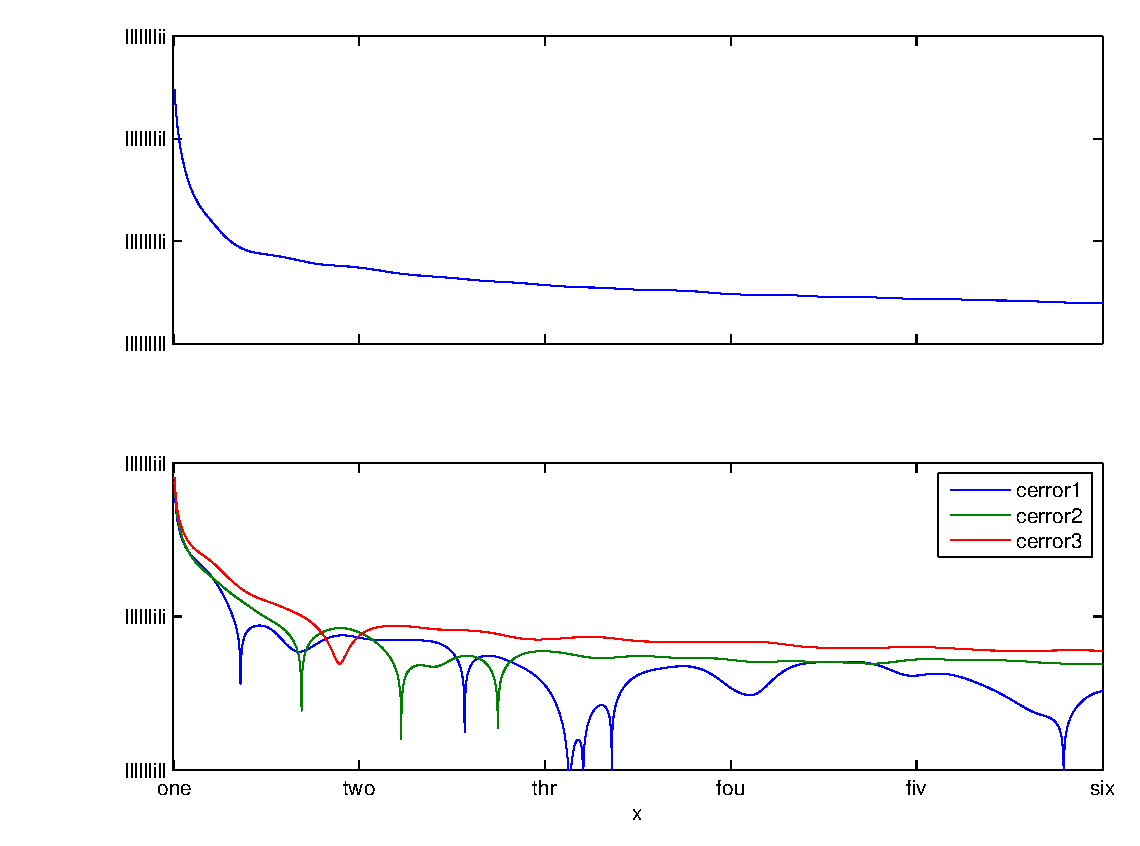
\includegraphics[width=\textwidth]{fig/mass_multi.eps}
				\label{fig:estim_mass_multi}
			\end{figure}
			Error of center of gravity $\vec{c} \left[\mathrm{m}\right]$
		\end{column}
		\begin{column}{0.5\textwidth}
			\centering
			\begin{figure}
				\psfrag{xaxis}[tr][br]{$t\left[\mathrm{s}\right]$}
				\psfrag{yaxis}[br][tr]{$\epsilon_{\scr{Inertia}}$}
				\psfrag{one}[c][Br]{$0$}
				\psfrag{two}[c][Br]{$1$}
				\psfrag{thr}[c][Br]{$2$}
				\psfrag{fou}[c][Br]{$3$}
				\psfrag{fiv}[c][Br]{$4$}
				\psfrag{six}[c][Br]{$5$}
				\psfrag{lllllllll}[Br][Bl]{$10^{-10}\  $}
				\psfrag{lllllllli}[Br][Bl]{$10^{-6}\  $}
				\psfrag{lllllllil}[Br][Bl]{$10^{-2}\  $}
				\psfrag{lllllllii}[Br][Bl]{$10^2\  $}
				\psfrag{Ierror1}[][]{\tiny \  $I_{xx,\scr{err}}$}
				\psfrag{Ierror2}[][]{\tiny \  $I_{yy,\scr{err}}$}
				\psfrag{Ierror3}[][]{\tiny \  $I_{zz,\scr{err}}$}
				\psfrag{Ierror4}[][]{\tiny \  $I_{xy,\scr{err}}$}
				\psfrag{Ierror5}[][]{\tiny \hspace{0.5cm} $I_{xz,\scr{err}}$}
				\psfrag{Ierror6}[][]{\tiny \hspace{0.5cm} $I_{yz,\scr{err}}$}
				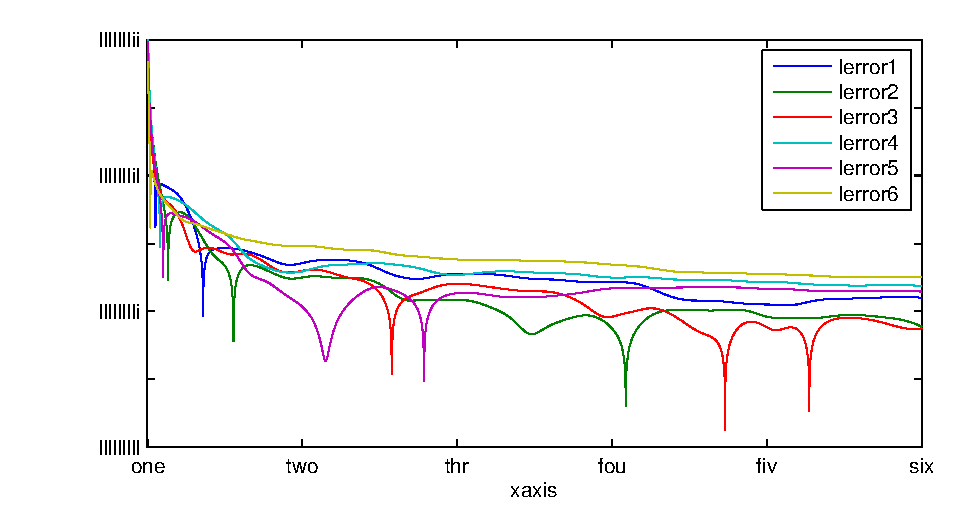
\includegraphics[width=\textwidth]{fig/inertia_multi.eps}
				\label{fig:estim_inertia_multi}
			\end{figure}
			Error of inertias $I \left[\mathrm{kg} \cdot \mathrm{m}^2\right]$
		\end{column}
	\end{columns}
\end{frame}

\begin{frame}
	%Benedikt
	\frametitle{Estimation Results with Noise ($P = \unit[0.05]{W}$)}
	\begin{columns}
		\centering
		\begin{column}{0.5\textwidth}
			\centering
			Error of mass $m \left[\mathrm{kg}\right]$
			\begin{figure}
				\psfrag{x}[tr][br]{$t\left[\mathrm{s}\right]$}
				\psfrag{y1}[br][tr]{$\epsilon_\scr{Mass}$}
				\psfrag{y2}[br][tr]{$\epsilon_\scr{CoM}$}
				\psfrag{one}[c][Br]{$0$}
				\psfrag{two}[c][Br]{$1$}
				\psfrag{thr}[c][Br]{$2$}
				\psfrag{fou}[c][Br]{$3$}
				\psfrag{fiv}[c][Br]{$4$}
				\psfrag{six}[c][Br]{$5$}
				\psfrag{lllllllll}[Br][Bl]{$10^{-6}\  $}
				\psfrag{lllllllli}[Br][Bl]{$10^{-4}\  $}
				\psfrag{lllllllil}[Br][Bl]{$10^{-2}\  $}
				\psfrag{lllllllii}[Br][Bl]{$10^0\  $}
				\psfrag{llllllill}[Br][Bl]{$10^{-10}\  $}
				\psfrag{llllllili}[Br][Bl]{$10^{-5}\  $}
				\psfrag{lllllliil}[Br][Bl]{$10^0\  $}
				\psfrag{cerror1}[][]{\tiny $c_{x,\scr{err}}$}
				\psfrag{cerror2}[][]{\tiny $c_{y,\scr{err}}$}
				\psfrag{cerror3}[][]{\tiny $c_{z,\scr{err}}$}
				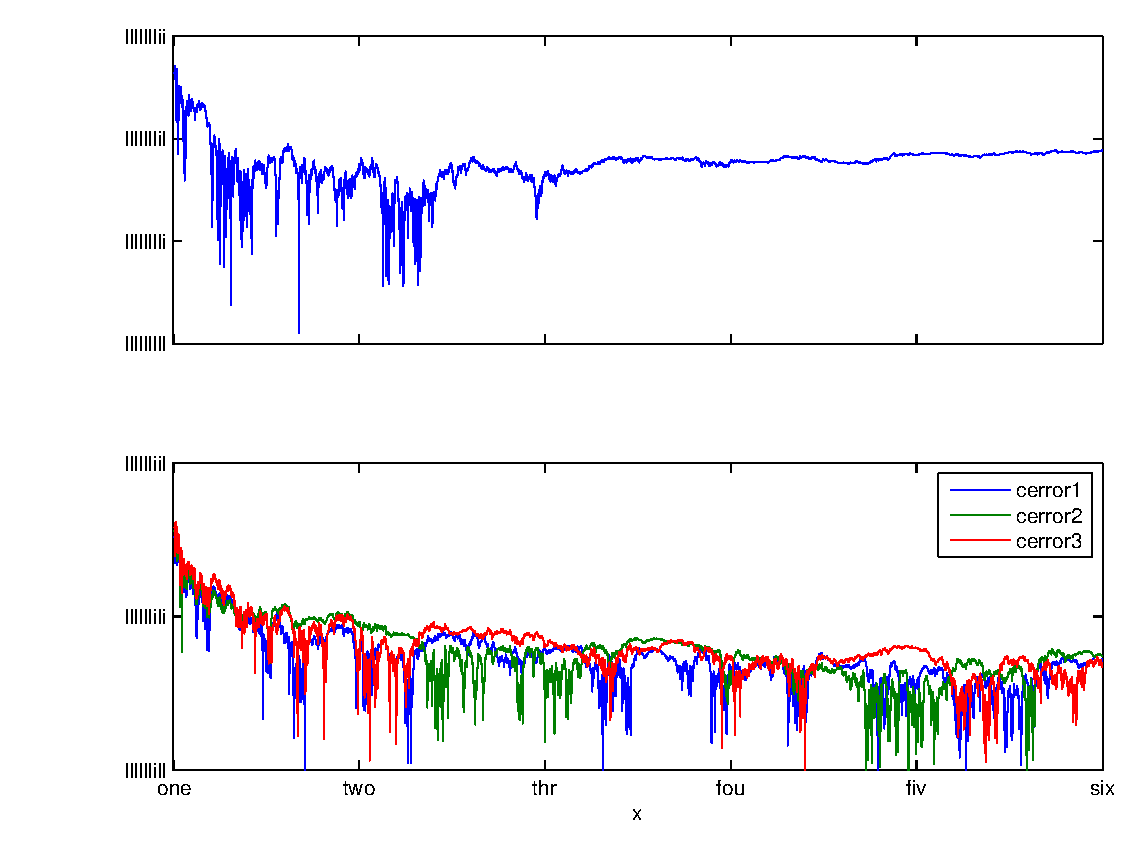
\includegraphics[width=\textwidth]{fig/mass_multi_noise.eps}
			\end{figure}
			Error of center of gravity $\vec{c} \left[\mathrm{m}\right]$
		\end{column}
		\begin{column}{0.5\textwidth}
			\centering
			\begin{figure}
				\psfrag{xaxis}[tr][br]{$t\left[\mathrm{s}\right]$}
				\psfrag{yaxis}[br][tr]{$\epsilon_{\scr{Inertia}}$}
				\psfrag{one}[c][Br]{$0$}
				\psfrag{two}[c][Br]{$1$}
				\psfrag{thr}[c][Br]{$2$}
				\psfrag{fou}[c][Br]{$3$}
				\psfrag{fiv}[c][Br]{$4$}
				\psfrag{six}[c][Br]{$5$}
				\psfrag{lllllllll}[Br][Bl]{$10^{-10}\  $}
				\psfrag{lllllllli}[Br][Bl]{$10^{-6}\  $}
				\psfrag{lllllllil}[Br][Bl]{$10^{-2}\  $}
				\psfrag{lllllllii}[Br][Bl]{$10^2\  $}
				\psfrag{Ierror1}[][]{\tiny \  $I_{xx,\scr{err}}$}
				\psfrag{Ierror2}[][]{\tiny \  $I_{yy,\scr{err}}$}
				\psfrag{Ierror3}[][]{\tiny \  $I_{zz,\scr{err}}$}
				\psfrag{Ierror4}[][]{\tiny \  $I_{xy,\scr{err}}$}
				\psfrag{Ierror5}[][]{\tiny \hspace{0.5cm} $I_{xz,\scr{err}}$}
				\psfrag{Ierror6}[][]{\tiny \hspace{0.5cm} $I_{yz,\scr{err}}$}
				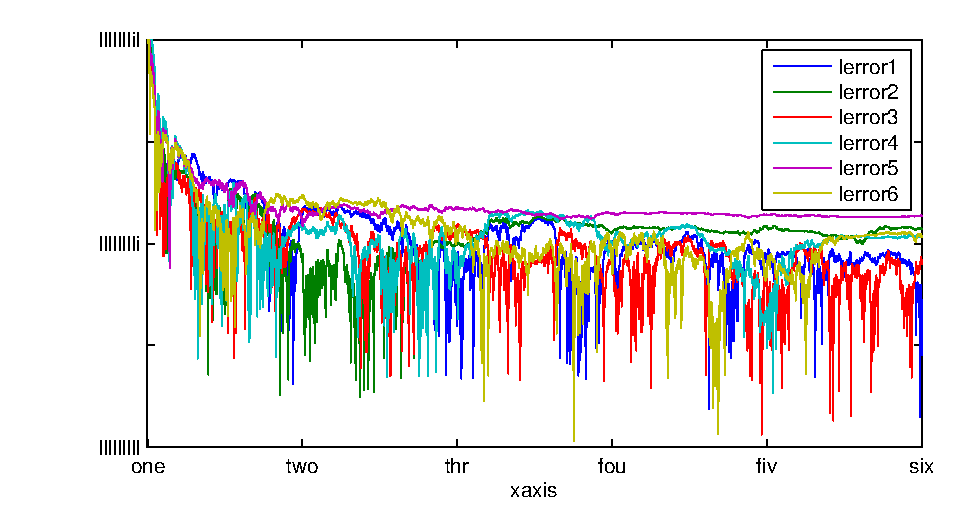
\includegraphics[width=\textwidth]{fig/inertia_multi_noise.eps}
			\end{figure}
			Error of inertias $I \left[\mathrm{kg} \cdot \mathrm{m}^2\right]$
		\end{column}
	\end{columns}
\end{frame}

\section{Outlook}
\begin{frame}
	%Benedikt
	\frametitle{Remaining Issues}
	\begin{itemize}
		\setlength{\itemsep}{10pt}
		\item Check if input values for the estimator are correct
		\item Find a good excitation pattern
		\item Incorporate human into the identification
	\end{itemize}
\end{frame}
\begin{frame}
	%Benedikt
	\frametitle{Time Schedule}
	\begin{tikzpicture}[node distance=0.2cm]
		\node[shape=circle,fill=green] (A) at (0, 0) {};
		\node[right=of A.east,anchor=west] {Get familiar with the topic and the hardware};
		\node[anchor=west] (DateA) at (0.2, -0.4) {19.11.2014};
		\draw[green,thick] (DateA) -- (A);
		\node[shape=circle,fill=tum_blue] (B) at (0, -1) {};
		\node[right=of B.east,anchor=west] {Implement load identification with one grasping point};
		\node[anchor=west] (DateB) at (0.2, -1.4) {5.12.2014};
		\draw[tum_blue,thick] (DateB) -- (B);
		\node[shape=circle,fill=tum_blue] (C) at (0, -2) {};
		\node[right=of C.east,anchor=west] {Implement load identification with more than one grasping point};
		\node[anchor=west] (DateC) at (0.2, -2.4) {19.12.2014};
		\draw[tum_blue,thick] (DateC) -- (C);
		\node[shape=circle,fill=tum_blue] (D) at (0, -3) {};
		\node[right=of D.east,anchor=west] {Trigger additional excitation by the human through the wrist band};
		\node[anchor=west] (DateD) at (0.2, -3.4) {16.01.2015};
		\draw[tum_blue,thick] (DateD) -- (D);
		\path[top color=green, bottom color=tum_blue, shading path={draw=transparent!0, very thick}] (A.south) -- (B.north);
		\draw[tum_blue,very thick] (B.south) -- (C.north);
		\draw[tum_blue,very thick] (C.south) -- (D.north);
	\end{tikzpicture}
\end{frame}

\appendix
\begin{frame}
	\frametitle{References}
	\printbibliography
\end{frame}

\end{document}